\begin{chapter}{Introduzione}

Negli ultimi anni la conoscenza \`e diventata il fattore pi\`u importante nel definire lo 
standard di vita; infatti la maggioranza delle economie avanzate tecnologicamente sono
basate sulla conoscenza. Quindi risulta essere fondamentale rendere la conoscenza una 
risorsa controllabile, replicabile e diffondibile.

Tuttavia la conoscenza \`e presente in pi\`u forme: codificata e tacita. La prima pu\`o facilmente
essere affidata ad un documento, ad un algoritmo, ad un codice o comunque traducibile in forme
esplicite e trasmissibili ad altri perch\`e ben strutturata. Quella tacita, invece, \`e difficile da 
acquisire, valutare e trasferire ad altri; ma \`e anche la pi\`u pregiata, \`e alla base del vantaggio 
competitivo ed \`e meno soggetta ad imitazioni.

Da queste esigenze nasce il \textit {knowledge management}, una disciplina mana\-geriale che studia la
conoscenza organizzativa e si occupa di individuare le metodologie e gli strumenti atti alla
sua gestione, con un approccio basato sull'innovazione: culturale, organizzativa e tecnologica.
Le ICT, \textit {Information and Communication Technologies}, svolgono un ruolo fondamentale di 
supporto per il knowledge management, fornendo tecnologie per la rappresentazione,
la condivisione e la creazione della conoscenza.

\begin{figure}[!htb]
	\centering
	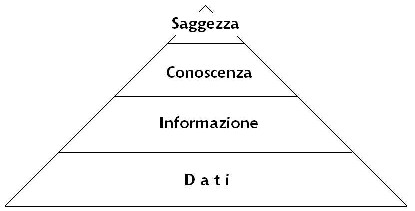
\includegraphics[scale=1.9]{img/piramidepic.png}
	\caption{Schema della gerarchia piramidale del knowledge management}
	\label{fig:piramidepic}
\end{figure}

Come possiamo notare dall'immagine, occorrono diversi raffinamenti prima di arrivare alla conoscenza.
I dati sono materiale grezzo, ovvero numeri e parole relativi a propriet\`a del reale, possono essere sintetizzati ed 
elaborati; in questo modo si ottiene informazione, ovvero dati interpretati, organizzati, contestualizzati e 
oggettivizzati. Infine si passa alla conoscenza, ovvero un insieme dinamico di esperienze concrete, valori,
informazioni ed intuizioni che consente la valutazione e l'inclusione di nuove esperienze ed informazioni.
In altre parole la conoscenza \`e informazione rielaborata ed applicata alla pratica.

\textit {Quindi, qual \`e la sfida per gli informatici?} La sfida consiste nel rappresentare, gestire, 
distribuire e manutenere sia conoscenza codificata che tacita. Questo mediante \textit {l'ingegneria della conoscenza}, 
una disciplina che si occupa dello studio e l'applicazione di metodologie e formalismi per la progettazione e la
realizzazione di \textit {sistemi basati su conoscenza}. 

\begin{section}{Agenti intelligenti}
I sistemi basati su conoscenza sono sistemi artificiali che hanno conoscenza 
del loro obiettivo, del contesto in cui operano e dell'affidabilit\`a della conoscenza su cui operano.
Nel caso in cui utilizzino una rappresentazione esplicita della conoscenza relativa al problema da risolvere,
si parla di \textit{agenti basati su conoscenza}. Questi sono \textit {software che portano a
termine compiti utili}, e sono caratterizzati dell'essere:
\begin{itemize}
    \item \textit {autonomi}, poich\`e l'azione che svolgono \`e guidata da regole e direttive interne;
    \item \textit {reattivi}, in quanto percepiscono aspetti dell'ambiente che li circonda e reagiscono in maniera appropriata;
    \item \textit {proattivi}, poich\`e possono prendere iniziative, intraprendendo azioni in funzione di obiettivi;
    \item \textit {sociali}, in quanto comunicano con altri agenti;
\end{itemize}
Ed \`e proprio grazie a queste caratteristiche \`e possibile parlare di \textit {agenti intelligenti},
dove l'intelligenza \`e descrivibile in termini di conoscenza posseduta dall'agente.
Questi agenti possiedono notevoli livelli di autonomia e agiscono nel loro ambiente in
maniera \textit{soddisfacente, razionale, flessibile}, anche in casi in cui le informazioni
disponibili siano parziali o incerte, esibendo un comportamento intelligente, consapevole, talvolta mostrando
una vera esperienza nel dominio in cui operano.

Esistono diverse applicazioni di questi sistemi: diagnosi e classificazioni, scheduling
di processi produttivi, controllo di robot in situazioni difficili e scarsamente strutturate,
controllo di veicoli autonomi, sistemi cooperativi, filtraggio e categorizzazione di
informazioni presenti sul web e non solo. Tutti questi sistemi apparentemente differenti
hanno molto in comune: un modello dell'ambiente, la possibilit\`a di passare
dall'osservazione all'evidenza, strategie d'azione, apprendimento dalle esperienze passate.
Ma ci\`o che li contraddistingue \`e \textit{la capacit\`a di fare inferenze}, che rende
possibile l'esibizione di un comportamento intelligente. 

L'inferenza \`e un procedimento che a partire da un insieme di \textit{fatti}, ovvero dati
che rappresentano accuratamente specifiche propriet\`a di un dominio, e di \textit{leggi}
(o regole), ovvero regole formali che rappresentano la dinamica del dominio, fa conseguire
nuovi fatti e regole. Per realizzare questa caratteristica \`e necessario un
\textit{meccanismo automatico di inferenza}, o \textit{motore inferenziale}, che si
definisce tramite un meta-interprete della conoscenza, e si realizza in un opportuno linguaggio
(o ambiente) di programmazione.

Quindi affinch\`e una macchina abbia conoscenza e sia in grado di esibire un comportamento intelligente
\`e fondamentale che la conoscenza sia fornita in maniera computabile. Per questo motivo, al fine di costruire
agenti basati su conoscenza \`e necessario definire il dominio, decidere il vocabolario dei predicati, delle variabile
e delle costanti, codificare la conoscenza generale dcondivisa del dominio, codificare una descrizione della 
specifica istanza del problema, e fornire interrogazioni alla procedura di inferenza.   
\end{section}

\begin{section}{Programmazione euristica}
\label{sec:heuristic-programming}
Per realizzare quanto detto finora, la programmazione algoritmica e il modello della macchina di Turing non sono
sufficienti. Viene quindi introdotta la \textit{programmazione euristica}, ramo della computer programming, che fa
uso di \textit{euristiche}, ovvero regole di senso comune derivate dall'esperienza, per risolvere problemi. Tutto ci\`o 
\`e in netto contrasto con la programmazione algoritmica, la quale si basa su procedure matematicamente dimostrabili.
La programmazione euristica invece, permette di definire programmi che risolvono problemi in maniera \textit{automatica}, 
senza un algoritmo definito a priori e tradotto in una sequenza di operazioni da eseguire. Inoltre molti sistemi esperti usano la programmazione euristica.

Nella programmazione euristica l'attenzione si \`e focalizzata, prima che su
metodi e tecniche per rappresentare, manipolare ed elaborarre la conoscenza, su:
\begin{itemize}
	\item \textit{Problem solving}: metodi di per costruire programmi in grado di
    raggiungere obiettivi spesso indeterminati e incerti (per maggiori dettagli si
    veda l'appendice \ref{sec:problem-solving});
	\item \textit{Metodi di ricerca}: metodi che generano tutte le possibili
    soluzioni e le verificano tutte fino a trovarne una adeguata.
\end{itemize}  

Un esempio di problemi che richiedono questo tipo di approccio solutivo sono i giochi
(ad esempio il gioco dell'otto, di cui \`e presente una breve descrizione nell'appendice
\ref{sec:gioco-filetto}), che andrebbero affrontati con metodi \textit{a tentativi};
in questi casi definire una soluzione equivale a ricercare una soluzione nello spazio
dei possibili stati del problema. Quindi \`e necessario rappresentare lo spazio di tutti i
possibili stati del problema, inteso come insieme di tutte le configurazioni possibili,
e va definita l'evoluzione da uno stato ad un altro mediante l'applicazione di operazioni
e regole; vanno inoltre definiti lo stato iniziale e gli stati obiettivo che rappresentano
le possibili soluzioni del problema. Il problema viene risolto mediante la ricerca, ovvero
l'esplorazione dello spazio degli stati per trovare un cammino solutivo, che consenta di
selezionare le appropriate operazioni (o regole) da applicare per arrivare alla soluzione.
\end{section}

\begin{section}{ANT - Another Non-trivial Tool}
ANT, acronimo di \textit{Another Non-trivial Tool}, \`e un tool per lo sviluppo di sistemi basati su conoscenza 
orientato alla risoluzione di giochi. Basato sul modello computazionale dei sistemi di produzione e implementato in C++,
mette a disposizione un linguaggio per la codifica della conoscenza basato sul meccanismo di attivazione delle regole
forward chaining. Nei paragrafi successivi vengono illustrati il modello di calcolo e le motivazioni che ci hanno
portato alla scelta del sopracitato linguaggio.
\end{section}
 
\begin{section}{Modello computazionale}
Il modello computazionale scelto \`e il \textit{il sistema a produzioni} \cite{Jackson99}. Un sistema a
produzioni \`e composto da
\begin{itemize}
    \item una lista ordinata di regole
    \item un interprete di regole che decide quando e quale regola applicare
    \item una memoria di lavoro (working memory), o database globale, che contiene i dati
    che rappresentano lo stato attuale del problema; la working memory viene modificata
    attraverso l'applicazione delle regole.
\end{itemize}

\noindent Le regole di produzione sono della forma:

\begin{figure}[!htb]
	\centering
	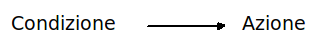
\includegraphics[scale=1.0]{img/formaregole.png}
	\caption{Forma delle regole di produzione}
	\label{fig:formaregole}
\end{figure}

\noindent Nella parte condizione, detta anche \textit{parte sinistra} (LHS, left hand side),
troviamo congiunzioni di letterali booleani che rappresentano l'insieme degli
stimoli percepiti dall'agente; mentre nella parte azione, o \textit{parte destra}
(RHS, right hand side), troviamo le modifiche da apportare all'ambiente
affinch\'e l'ambiente produca nuovi stimoli.  

Il ruolo della working memory \`e di contenere dati nella forma
\textit{attributo-valore}. Questi dati vengono utilizzati dall'interprete per scegliere
quali regole attivare o eseguire in base alla presenza o all'assenza di determinati dati
che soddisfino la condizione di una o pi\`u regole. 

L'interprete per le regole di produzione pu\`o essere descritto in termini di cicli \textit{recognize-act} (riconosci-agisci)
che \`e composto dei seguenti passi:

\begin{itemize}
    \item \textit{matching}: viene verificata la corrispondenza tra la parte sinistra delle regole
          e i dati presenti nella working memory;
    \item \textit{risoluzione dei conflitti}: se ci sono pi\`u regole che possono essere eseguite,
          ne viene scelta una secondo un qualche criterio;
    \item \textit{applicazione della regola}: \`e possibile che venga aggiunto, rimosso o modificato
          un elemento della working memory; dopo questa azione, quindi, si ritorna al passo 1.
\end{itemize}

L'esecuzione si ferma se nessuna regola \`e attiva, oppure se la parte destra di una regola
contiene un comando esplicito per la terminazione. Generalmente, nei sistemi di produzioni,
esistono diverse modalit\`a di attivazione delle regole:
\begin{itemize}
    \item \textit{Forward Chaining} (o concatenazione in avanti): se l'attivazione delle regole
    \`e fatta mediante il matching degli antecedenti con gli elementi della working memory;
    \item \textit{Backward Chaining} (o concatenazione all'indietro): se l'attivazione delle
    regole \`e fatta mediante il matching della parte destra della regola con l'obiettivo che si
    intende raggiungere.
\end{itemize}
\`E interessante notare che il momento di analisi dei dati \`e nettamente separato dal
momento di elaborazione o di modifica dei dati; inoltre alla memoria di lavoro possono
accedere tutte le regole. In aggiunta le regole non ``non chiamano'' altre regole, ma
la connessione degli operatori avviene mediante la memoria di lavoro. \`E altrettanto
importante notare che i sistemi di produzione consentono uno sviluppo incrementale,
ovvero non c'\`e alcun problema nel togliere o aggiungere regole di produzione mantenendo
la coerenza tra di esse (non ambiguit\`a).

Infine \'e possibile individuare un ulteriore classificazione di questi sistemi:
\begin{itemize}
    \item \textbf{Reaction system}: se la parte sconseguente delle regola prevede un'azione;
    \item \textbf{Deduction system}: se la parte sconseguente delle regola prevede una nuova asserzione.
\end{itemize}

	\begin{subsection}{Il problema del matching} 
	Il matching \`e un operazione pesante e strettamente connessa alla complessit\`a della
    rappresentazione del problema; talvolta pu\`o risultare un problema np-completo.
    Questo perch\`e richiede che sia ripetuto su tutte le regole affinch\`e vengano individuate
    tutte le regole applicabili. Ne consegue una ricerca esaustiva tra tutte le regole che
    risulta essere inefficiente e computazionalmente pesante. Quindi il problema richiede
    efficienti algoritmi di matching, in particolar modo per il matching con variabili,
    e la possibilit\`a di ricerca con meccanismi di selezione.

    Inoltre non sempre le precondizioni di una regola sono soddisfatte da un particolare
    stato. Questo tipo di problema \`e poco sentito se le precondizioni vengono definite
    con costanti; diventa invece complesso in presenza di variabili.
	\end{subsection}

	\begin{subsection}{Graph Search}
	Nei sistemi a produzione il problema centrale \`e scegliere una regola applicabile. Una
    caratteristica importante di questa operazione \`e la quantit\`a di conoscenza utilizzata
    nella selezione dalla strategia di controllo. Quindi la ricerca nello spazio degli stati
    pu\`o essere pi\`u o meno informata. Infatti abbiamo:

	\begin{itemize}
	    \item \textit{ricerca cieca}: ricerca sistematica ed esaustiva dello spazio degli
              stati del problema;
	    \item \textit{ricerca informata euristicamente}: ricerca che fa uso di
              conoscenza per ridurre drasticamente lo spazio di ricerca e trovare un cammino ottimale. 
	\end{itemize}

	Generalmente, per realizzare un \textit{meccanismo di inferenza} (o
    interprete di regole) di un sistema a produzioni \`e quello di dotarlo di
    una \textit{graph search} che gli consenta di esplorare lo spazio di ricerca
    per determinare un cammino ottimale. Infatti il problema di trovare una
    sequenza di regole che trasformino un stato del prblema in un altro \`e
    equivalente a trovare un cammino su un grafo orientato in cui ogni nodo
    rappresenta uno stato del problema ed ogni arco una regola che fa passare
    da uno stato ad un altro. Inoltre nella ricerca \`e importante:

	\begin{itemize}
	    \item il modo in cui si rappresentano gli stati del problema, ovvero i
              nodi del grafo su cui organizzare la ricerca;
	    \item la direzione in cui si intraprende la ricerca;
	    \item il modo in cui si selezionano le regole applicabili (efficienza del matching). 	
	\end{itemize}
	\end{subsection}
	  	
	\begin{subsection}{Costi ed efficienza}
	L'efficienza computazionale di un sitema a produzioni dipende da dai costi
    computazionali della strategia di controllo. 
	\begin{figure}[!htb]
	\centering
	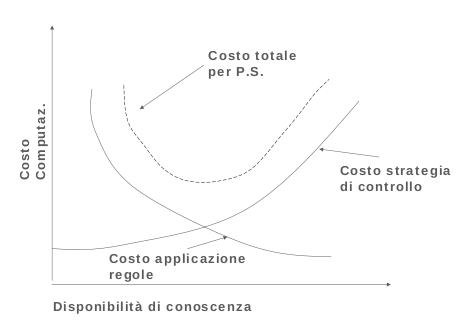
\includegraphics[scale=0.9]{img/costoapplicazioneregole.png}
	\caption{Costo per un production system}
	\label{fig:costoapplicazioneregole}
	\end{figure}
	
	Come possiamo notare dalla figura \ref{fig:costoapplicazioneregole}, i costi dipendono
    dal \textit{costo di applicazione delle regole} e dai \textit{costi di controllo}.
    Inoltre \`e evidente che:

	\begin{itemize}
	    \item ad un estremo, poca conoscenza disponibile implica che la selezione delle
        regole \'e fatta in maniera arbitraria, e quindi un basso costo di controllo
        implica un alto costo di attivazione delle regole;
	    \item all'altro estremo, una conoscenza pi\`u approfondit del problema consente
        di scegliere la regola giusta al momento giusto; quindi alto costo di controllo
        implica basso costo di attivazione delle regole. 	
	\end{itemize}  	
	\end{subsection}
\end{section} 


\begin{section}{Scelta del linguaggio}
ANT \`e scritto in C++. Questa scelta \`e motivata in larga parte dal fatto che
il C++ sia un linguaggio ad oggetti e, come sappiamo, tale paradigma mette a disposizione il concetto 
di astrazione di classe, che ben si presta ad essere considerato per la gestione di un 
sistema di questo tipo. Tuttavia, prima di consacrare il C++ come linguaggio scelto, 
sono stati valutati altri linguaggi come C, Java e Python.

Di fatto, abbiamo scartato subito Java. Nonostante sia un linguaggio orientato
agli oggetti, presenta due notevoli problemi:

\begin{enumerate}
	\item non \`e compilato: questo, in realt\`a, non \`e del tutto vero in quanto
	      Java \`e un linguaggio byte-compilato, ovvero il prodotto del compilatore
				\`e un file che non contiene istruzioni in linguaggio macchina per 
				l'architettura nativa, bens\`i un ``bytecode'' che pu\`o essere
				interpretato solo da una Java Virtual Machine, che per\`o \`e disponibile
				per una moltitudine di piattaforme e, di fatto, rende compatibile lo stesso
				eseguibile per pi\`u sistemi operativi su architetture differenti. Tuttavia
				la JVM aggiunge uno strato di complessit\`a non indifferente dovendo infatti
				traslare le istruzioni dal bytecode al linguaggio macchina. Tralaltro nella
				maggior parte dei casi non c'\`e una corrispondenza uno-ad-uno tra il bytecode
				e il linguaggio macchina (essendo disponibile il processo di traslazione anche per
				architetture diverse dall'x86 usato nei normali calcolatori\footnote{con questa
				espressione intendiamo che l'architettura x86 \`e la pi\`u diffusa nell'ambito
				del personal computing e recentemente ha incrementato la quota di mercato anche
				in ambito server, ma certamente non \`e l'unica: \`e molto probabile, infatti,
				che dispositivi embedded montino processori ARM o Motorola Z80 la cui architettura,
				e quindi anche il rispettivo linguaggio macchina, \`e totalmente diversa da quella
				dell'x86}) pertanto questa operazione non pu\`o, per ovvi motivi, avere tempo costante.
				Negli ultimi anni questo processo ha subito notevoli miglioramenti grazie all'introduzione
				di tecniche di \textit{just in time compilation} \cite{367714} ma, per i
				nostri scopi, questa genere di implementazione \`e un collo di bottiglia non
				indifferente.

	\item la gestione della memoria: in Java la memoria \`e gestita attraverso un
	      processo di \textit{garbage collection}, ovvero l'allocazione e deallocazione
				della memoria \`e una cosa che viene gestita direttamente dalla virtual
				machine tramite l'utilizzo di un sistema di reference counting (ogni oggetto
				che utilizza quella determinata area di memoria incrementa un contatore, che
				viene decrementato non appena l'oggetto in questione non ha pi\`u bisogno di
				utilizzare la memoria allocata; quando questo contatore giunge a zero la
				memoria potr\`a allora essere deallocata) Se per moltissimi ambiti questo
				pu\`o essere solo un vantaggio in quanto riduce la complessit\`a del programma,
				per i nostri scopi questo \`e un problema non indifferente data la grande
				quantit\`a di memoria che viene utilizzata durante l'esecuzione. Inoltre, il
				comportamento della JVM sino alla versione 5, per i nostri scopi, era disastroso
				in termini di performance. Difatti, fino a quella versione, si adottava come
				politica di gestione di garbage collection, quella della non-deallocazione.
				Ovvero la memoria veniva continuamente allocata fino a quando non ce ne era pi\`u
				disponibile. Solo allora veniva invocata la garbage collection che, di fatto,
				bloccava per un certo periodo di tempo l'esecuzione del programma fintanto
				che la memoria non pi\`u utilizzata (ovvero quei blocchi per cui il reference
				counting era giunto a zero) veniva liberata.
\end{enumerate}

Per il Python e il C gli argomenti sono stati meno forti. Rispettivamente, l'impossibilit\`a
di eseguire direttamente il linguaggio macchina per il primo e la mancanza di un pieno
supporto alla programmazione ad oggetti per il secondo, hanno reso di fatto la scelta
del C++ obbligata. In sostanza la scelta del linguaggio si \`e basata su tre punti,
quello della necessit\`a di poter compilare realmente il programma, senza doverlo eseguire
all'interno di macchine virtuali di vario genere, la necessit\`a di dover gestire
manualmente le allocazioni e deallocazioni di memoria e il pieno supporto alla programmazione
ad oggetti.

\end{section}

\begin{section}{Perch\`e ANT?}
Come si \`e gi\`a detto in precedenza, ANT \`e l'acronimo di Another Non-trivial Tool;
\`e abbastanza intuitivo notare la forte contrapposizione tra i termini another (un'altro)
e non-trivial (non banale); infatti ANT \`e solo un altro strumento nel suo genere.
Tuttavia controllare il comportamento di un sistema a regole pu\`o essere un problema non
affatto banale. Citando Peter Jackson \cite{Jackson99}:\\

\quotation{\textit{``Controlling the behaviour of
rule-based systems can pose non-trivial problems''}}
\\

\noindent Ma, tralasciando l'acronimo, \textit{ant} in inglese vuol dire formica,
termine di paragone spesso usato per sottolineare la lentezza di qualcuno o qualcosa;
dando questa seconda accezione, abbiamo voluto esorcizzare il nostro timore riguardo
le prestazioni in termini di velocit\`a della nostra applicazione. 
\end{section}

\begin{section}{Perch\`e un motore inferenziale e non un sistema esperto}
La scelta \`e stata motivata dal fatto che la realizzazione di un motore inferenziale fa
convergere gran parte delle conoscenze acquisite durante tutto il percorso di studi durante
corsi quali quello di ``linguaggi di programmazione'', ``metodi avanzati di programmazione'',
``algoritmi e strutture dati'' ma non solo: teorie sui linguaggi formali, automi, algoritmi,
strutture dati, paradigmi di programmazione, design pattern, architettura dei moderni
calcolatori, matematiche, sono solo alcuni esempi di argomenti la cui utilit\`a
pu\`o essere messa in dubbio durante il corso di studio ma che invece sono addirittura
fondamentali (e non solo necessarie), ed un progetto quale quello da noi scelto ne mette
in risalto le diverse caratteristiche.

La prospettiva di doversi confrontare con problemi reali e complessi sia dal punto di vista
strettamente computazionale che dal punto di vista algoritmico \`e stata un ulteriore
spinta verso la scelta della realizzazione del motore inferenziale piuttosto che il sistema esperto.
\end{section} 

\end{chapter}
